\documentclass[10pt,landscape,a4paper] {extarticle}
\usepackage{amsmath}
\usepackage{graphicx}
\usepackage{float}
\usepackage{geometry}
\usepackage{multicol}
\usepackage{extsizes}
\geometry{left=1.0cm, right=1.0cm, top=1.0cm, bottom=1.0cm}

\begin{document}

\begin{multicols}{3}

\section{Radiometry}

\subsection{Radiant Energy}

The \textbf{Energy} of electromagnetic radiation. \\
\[
	Q[J=Joule]
.\] 

\subsection{Radiant Flux(Power)}

\textbf{Energy} per \textbf{Unit Time}.
\[
	\Phi \equiv \frac{dQ}{dt} [W=Watt] [lm=lumen]
.\] 

\subsection{Radiant Intensity} 

\textbf{Power} emitted per \textbf{Unit Solid Angle}.
\[
	I(\omega)\equiv\frac{d\Phi}{d\omega}
	\left [ \frac{W}{sr} \right ] \left [ \frac{lm}{sr}=cd=candela \right ]
.\] 

\subsection{Irradiance}

\textbf{Power} emitted or received per \textbf{Unit Area}.

\[
	E(x) \equiv \frac{d\Phi(x)}{dA}
	\left [ \frac{W}{m^2} \right ] \left [ \frac{lm}{m^2}=lux \right ]
.\] 

\subsection{Radiance}

(1)\textbf{Power} per \textbf{Unit Solid Angle} per \textbf{Projected Unit Area}.\\
(2)\textbf{Irradiance} per \textbf{Solid Angle}. (Incident Radiance)\\
(3)\textbf{Intensity} per \textbf{Projected Unit Area}. (Exiting Radiance)

\begin{figure}[H]
\centering
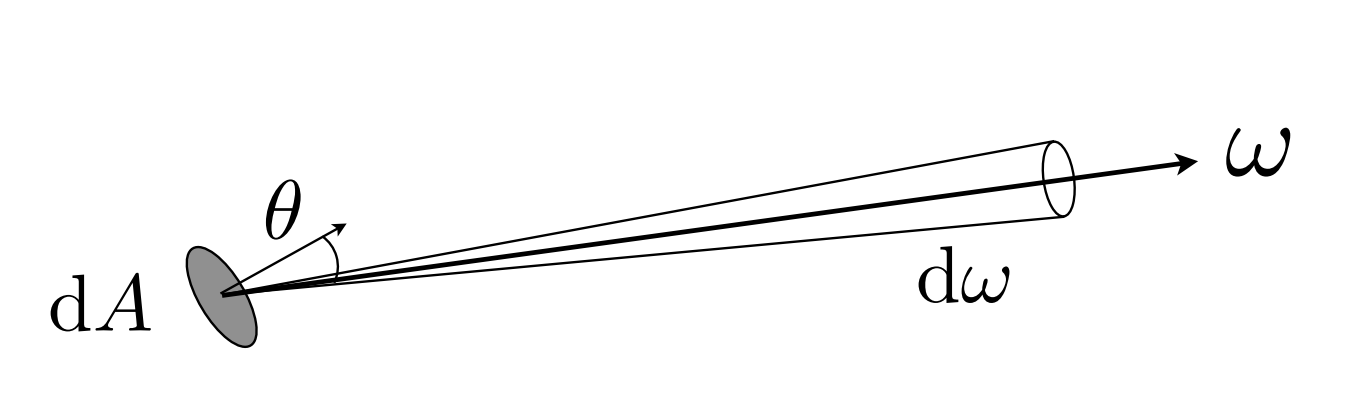
\includegraphics[width=5cm]{img/radiance.png}
\end{figure}

\begin{align*}
	L(p,\omega) &\equiv \frac{d^2\phi(p,\omega)}{d\omega dA cos\theta} 
	\left [ \frac{W}{sr\ m^2} \right ] 
	\left [ \frac{cd}{m^2} = \frac{lm}{sr\ m^2} = nit \right ] (1) \\
				&\equiv \frac{dE(p)}{d\omega cos\theta} \ (2)\\
				&\equiv \frac{dI(p,\omega)}{dA cos\theta} \ (3)
\end{align*}

\subsection{Irradiance vs. Radiance}
\textbf{Irradiance:} total power received by area $dA$ \\
\textbf{Radiance:} power received by area dA from "direction" $d\omega$

\begin{figure}[H]
\centering
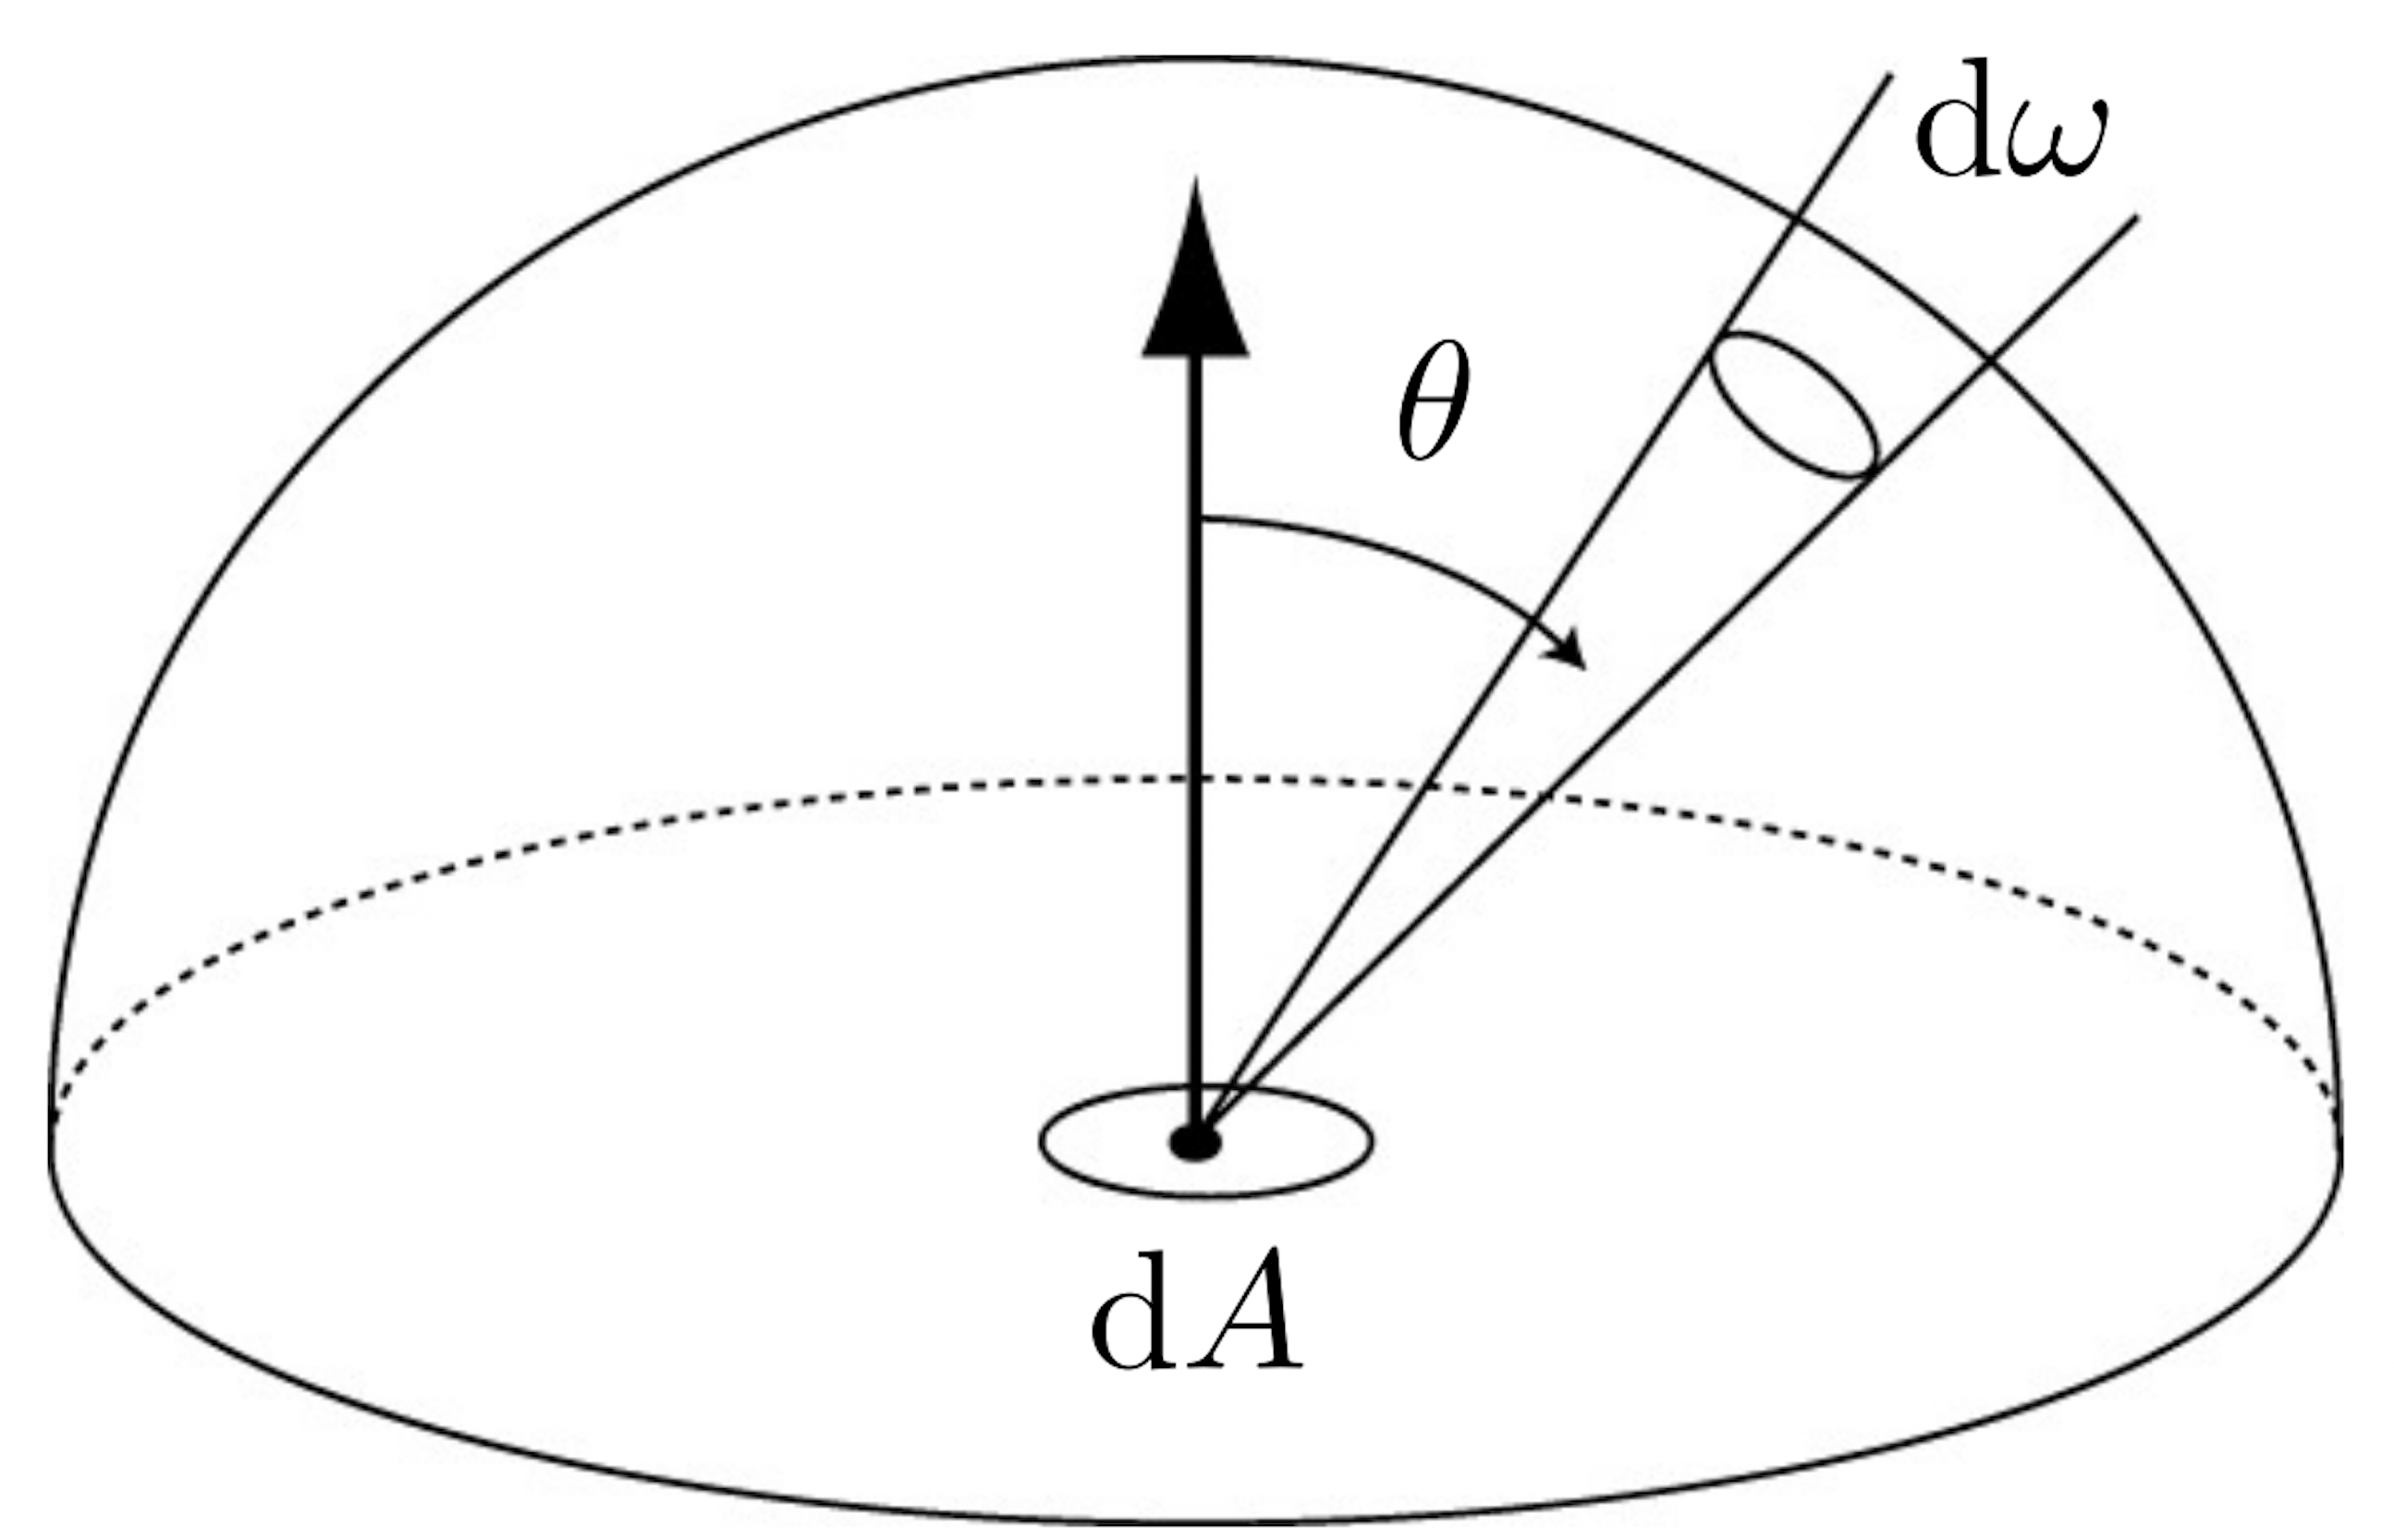
\includegraphics[width=3.5cm]{img/hemisphere_integral.png}
\end{figure}

\[
	dE(p,\omega) &= L_{i}(p,\omega)cos\theta d\omega
.\] 
\[
	E(p) &= \int_{H^2} L_i(p,\omega)cos\theta d\omega
.\] 

\section{BRDF}

\subsection{Reflection at a Point}

Radiance from direction $\omega_{i}$ turns into the power $E$ that $dA$ receives \\
Then power $E$ will become the radiance to any other direction $\omega_{o}$

\begin{figure}[H]
\centering
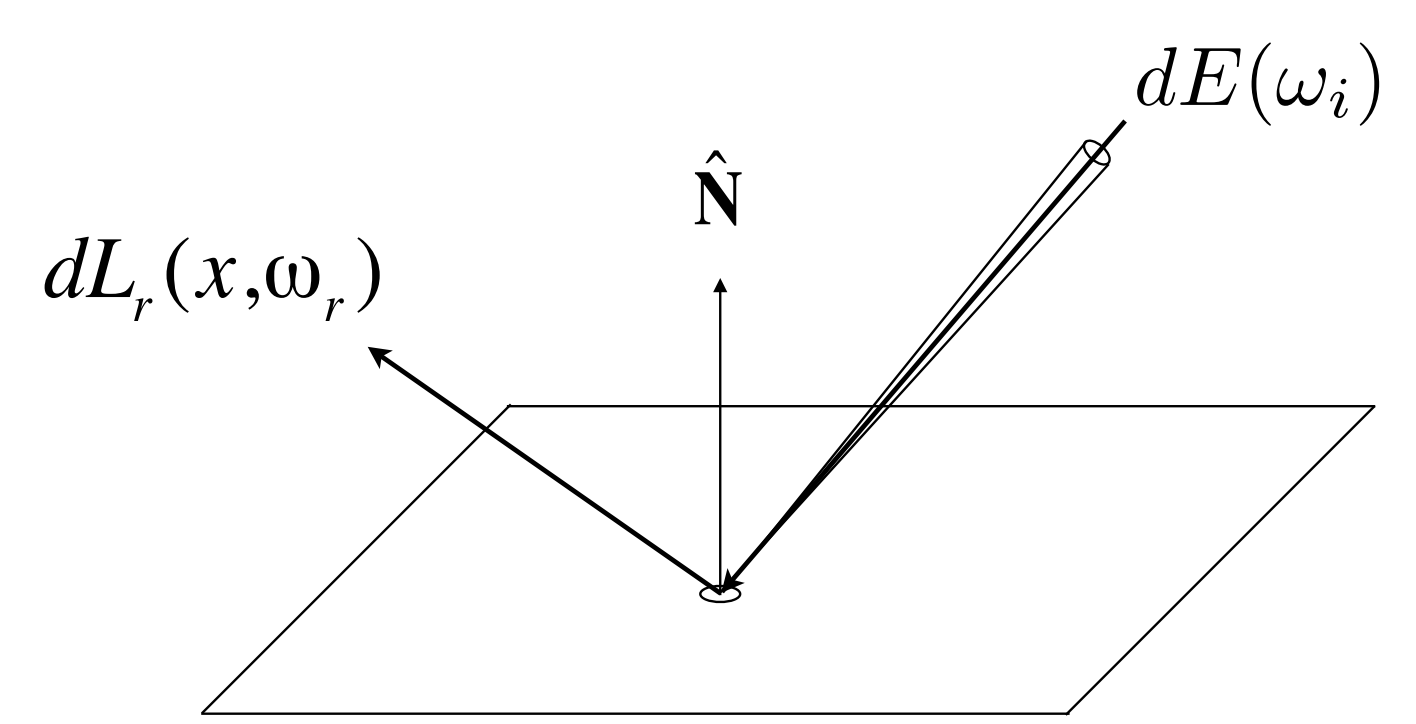
\includegraphics[width=5cm]{img/reflection.png}
\end{figure}

\paragraph{Differential Irradiance Incoming:} 
\[
	dE(\omega_{i}) = L(\omega_{i})cos\theta_{i}d\omega_{i}
.\]
\paragraph{Differential Radiance Exiting(due to $dE(\omega_{i})$):} 
\[
	dL_{r}(\omega_{r})
.\] 

\subsection{BRDF}

How much light is reflected into each outgoing direction $\omega_{r}$ from each incoming direction.

\begin{figure}[H]
\centering
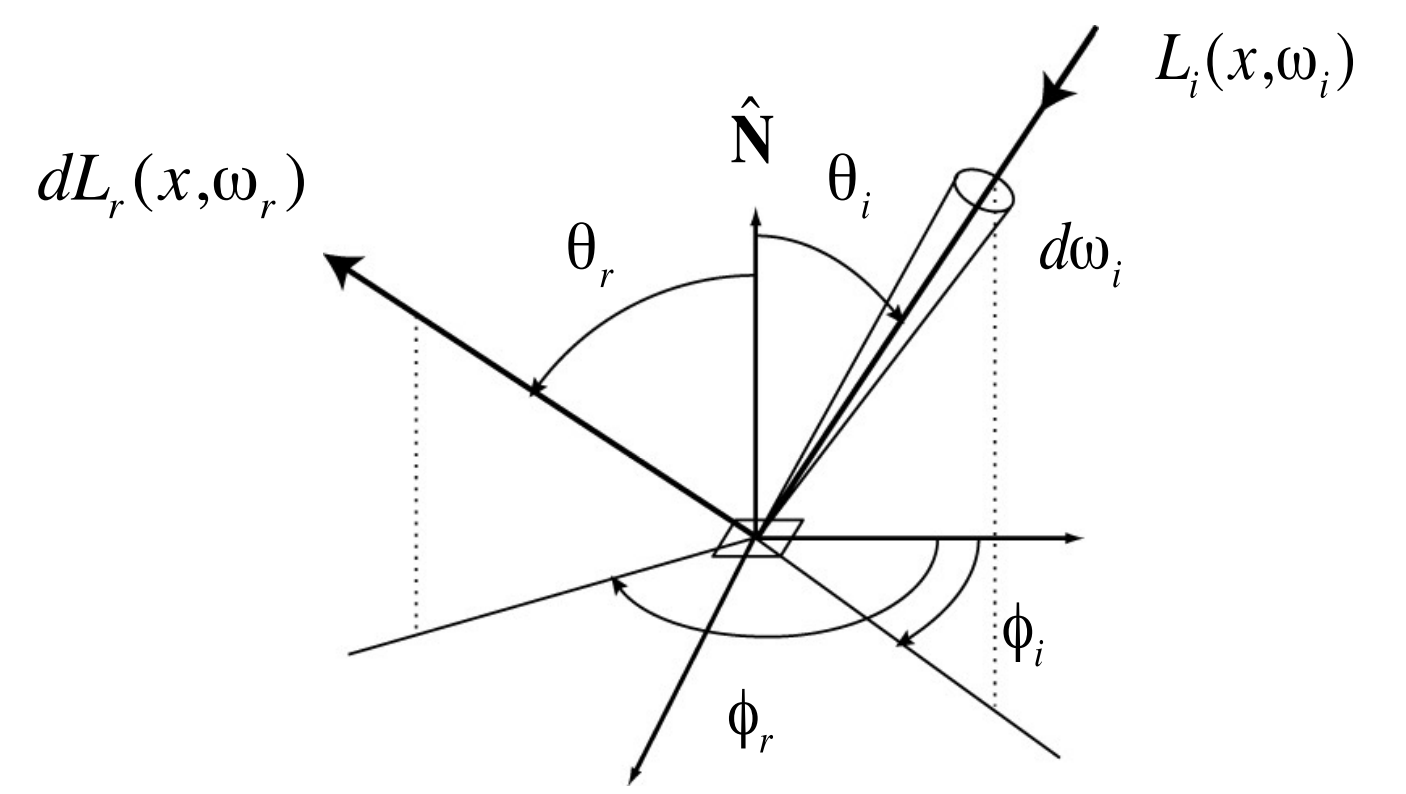
\includegraphics[width=6cm]{img/brdf.png}
\end{figure}

\[
	f_{r}(\omega_{i} \rightarrow \omega_{r}) 
	= \frac{dL_{r}(\omega_{r})}{dE_{i}(\omega_{i})}
	= \frac{dL_{r}(\omega_{r})}{L_{i}(\omega_{i})cos\theta_{i}d\omega_{i}}
	\left [ \frac{1}{sr} \right ]
.\] 

\subsection{Reflection Equation}

\begin{figure}[H]
\centering
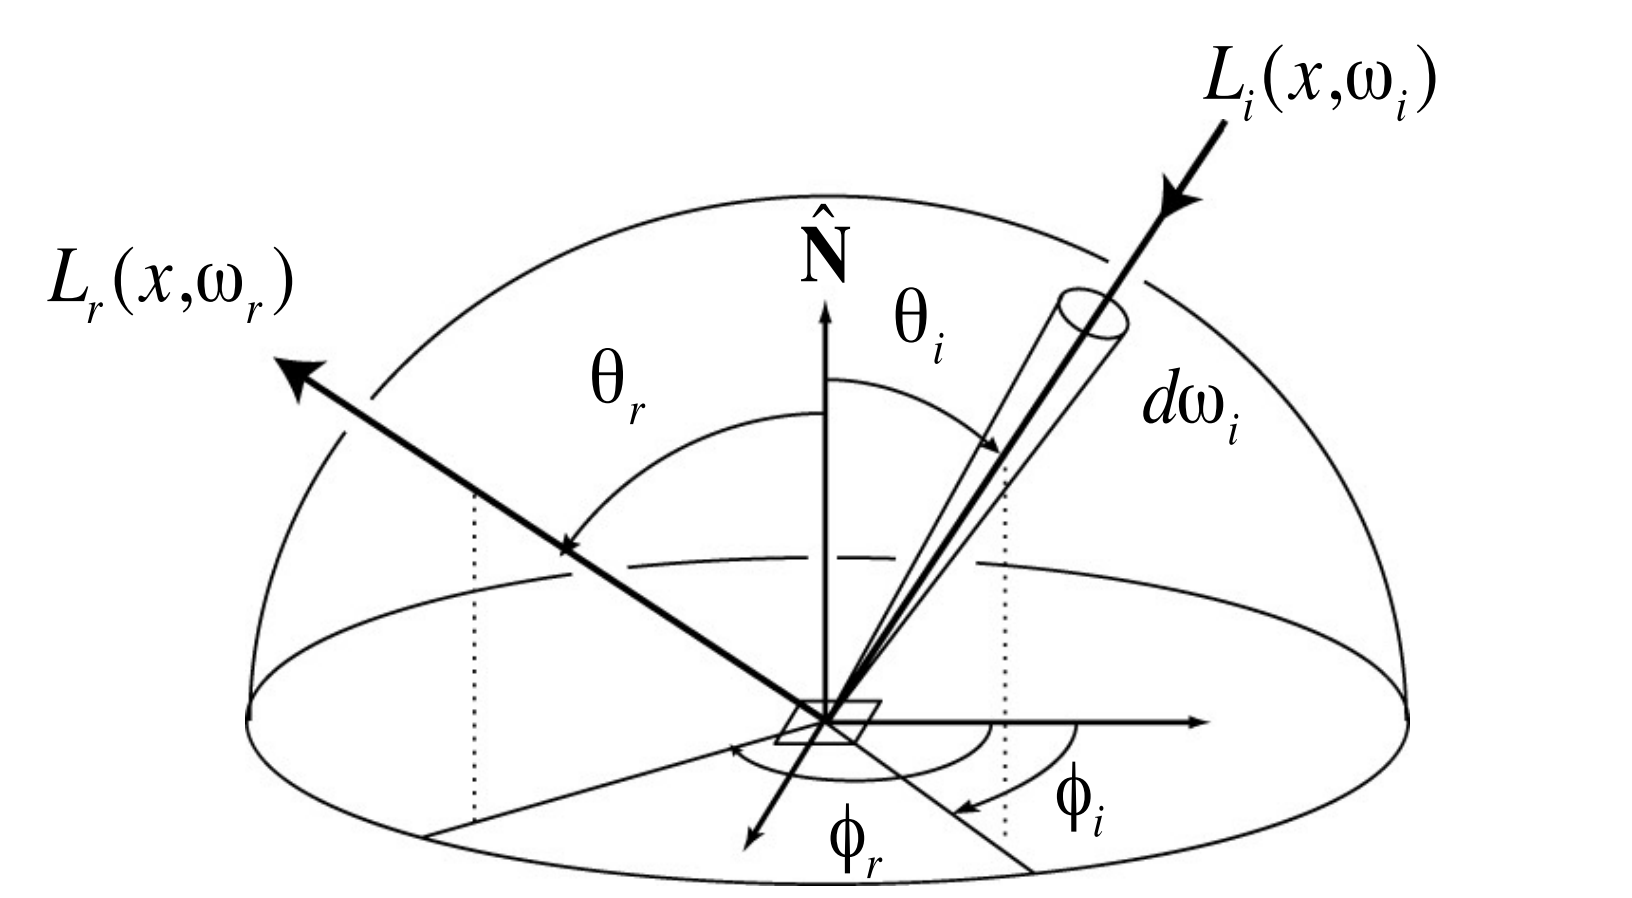
\includegraphics[width=6cm]{img/reflection_equation.png}
\end{figure}

\[
	L_{r}(p,\omega_{r}) = \int_{H^2} f_{r}(p,\omega_{i} \rightarrow \omega_{r}) L_{i}(p,\omega_{i})cos\theta_{i}d\omega_{i}
.\] 

\end{multicols}

\end{document}
